\documentclass[tikz,border=3pt]{standalone}
\usepackage[UTF8,fontset=windows]{ctex}
\usepackage{amsmath}
\definecolor{curveblue}{HTML}{245C86}
\begin{document}
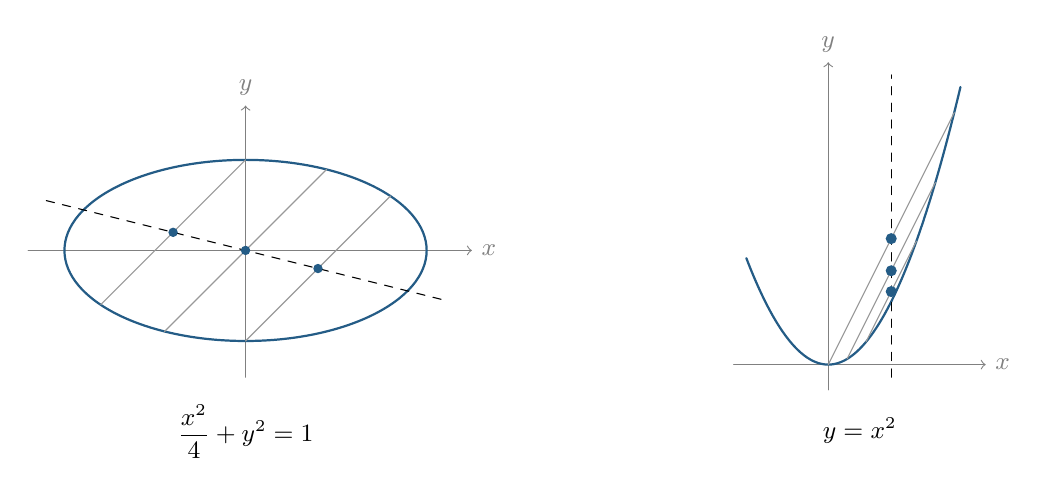
\begin{tikzpicture}[line cap=round,line join=round,font=\small]
\begin{scope}[x=1.15cm,y=1.15cm]
  \draw[->,gray] (-2.4,0)--(2.5,0) node[right] {$x$};
  \draw[->,gray] (0,-1.4)--(0,1.6) node[above] {$y$};
  \draw[curveblue,thick] (0,0) ellipse[x radius=2,y radius=1];
  \draw[dashed] (-2.2,.55)--(2.2,-.55);
  \foreach \h in {-.8,0,.8} {
    \pgfmathsetmacro{\t}{sqrt((1-5*\h*\h/16)*4/5)}
    \draw[gray!80] ({\h-\t},{-\h/4-\t})--({\h+\t},{-\h/4+\t});
    \fill[curveblue] (\h,{-\h/4}) circle[radius=1.7pt];
  }
  \node at (0,-2) {$\dfrac{x^2}{4}+y^2=1$};
\end{scope}
\begin{scope}[shift={(7.4,-1.45)},x=.8cm,y=.8cm]
  \draw[->,gray] (-1.5,0)--(2.5,0) node[right] {$x$};
  \draw[->,gray] (0,-.4)--(0,4.8) node[above] {$y$};
  \draw[curveblue,thick,domain=-1.3:2.1,samples=90] plot (\x,{\x*\x});
  \draw[dashed] (1,-.2)--(1,4.6);
  \foreach \t in {.4,.7,1} {
    \draw[gray!80] ({1-\t},{(1-\t)^2})--({1+\t},{(1+\t)^2});
    \fill[curveblue] (1,{1+\t*\t}) circle[radius=2pt];
  }
  \node at (.5,-1.05) {$y=x^2$};
\end{scope}
\end{tikzpicture}
\end{document}
